\section{Fiji VM}
I linguaggi più utilizzati, in genere, per sistemi real-time sono Ada e C (per i più coraggiosi C++). Tuttavia la complessità e la dimensione crescente del codice, unita alla disponibilità di tanti programmatori ben addestrati hanno portato fatto crescere l'interesse verso l'utilizzo di Java. Inoltre, dato che le applicazioni Android sono generalmente scritte in Java, per poter utilizzare quei dispositivi in contesti con vincoli temporali è necessario avvicinare il mondo Java e quello real-time. Per farlo è necessario sviluppare un runtime, e una GC, che siano prevedibili e adatti all'utilizzo in sistemi con vincoli temporali stretti. La Fiji VM (fVM) ha esattamente questo scopo. Figura\ref{fig:fijiarch} mostra la sua architettura.
\begin{figure}
	\centering
	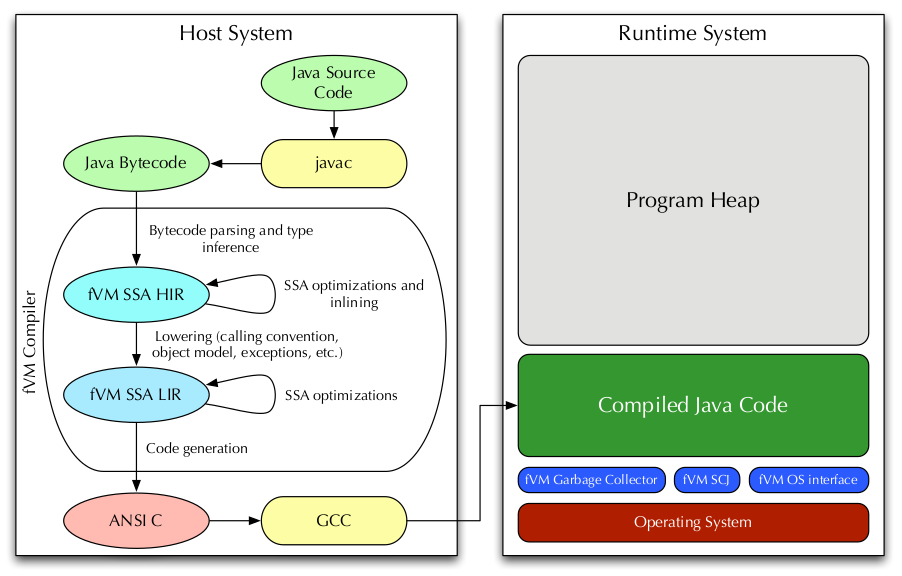
\includegraphics[width=0.9\linewidth]{fijiarch}
	\caption[Architettura di Fiji VM]{Architettura di Fiji VM}
	\label{fig:fijiarch}
\end{figure}

\subsection{Compilazione}
fVM utilizza un compilatore AOT per convertire codice Java in ANSI C. A partire dal codice Java vengono inizialmente effettuate diverse ottimizzazioni basate sulla rappresentazione static-single-assignment (SSA); tra queste troviamo:
\begin{itemize}
	\item inlining;
	\item devirtualizzazione (chiamate virtuali tradotte in chiamate dirette;
	\item virtualizzazione (chiamate di interfaccia in chiamate virtuali);
	\item eliminazione dei lock (se si sa che un lock è attivo non serve fare avere codice che lo attiva nuovamente);
	\item eliminazione dei controlli sulle dimensioni degli array e sui null pointers;
	\item copy propagation.
\end{itemize}
Di seguito vengono descritte le modalità di compilazione.

\paragraph{Null pointers} \mbox{} \\
Java controlla che ogni puntatore sia non null prima di utilizzarlo. Attraverso tecniche di analisi del flusso di controllo è possibile eliminare questi controlli ed evitare percorsi di esecuzione diversi con tempi diversi.

\paragraph{Dimensione degli array} \mbox{} \\
Così come per i controlli sui puntatori nulli, anche i controlli sugli indici degli array possono essere rimossi per evitare di incorrere in incrementi del tempo di esecuzione.

\paragraph{Controlli per la garbage collection} \mbox{} \\
Dato che il GC opera concorrentemente all'applicazione (= non la mette in pausa), è necessario fare alcuni controlli a run-time:
\begin{itemize}
	\item \textbf{sync-points}: indicano che lo stack del thread corrente deve essere analizzato dal GC;
	\item \textbf{stone barriers}: assicurano che le modifiche fatte allo heap siano viste dal GC.
\end{itemize}
I primi sono inseriti utilizzando una politica che assicura una distanza limitata tra due diversi punti. Questo significa che ogni ciclo ne avrà almeno uno. L'impatto sui cicli ''snelli'' è significativo, perché viene introdotto un nuovo branch. Tuttavia i test effettuati mostrano che, in generale, l'overhead è trascurabile. fVM mantiene un puntatore ad una struttura dati corrispondente allo del thread corrente. Questa struttura contiene un campo, \texttt{shouldSync}, che è \texttt{true} quando il thread deve sincronizzarsi (\texttt{yield()}). I thread con alta priorità, tale da poter prerilasciare il GC, non sono affetti da questo controllo, ma tutti gli altri subiranno un overhead inevitabile. 

Le seconde introducono un altro overhead nella pulizia, e vengono tradotte nel modo seguente (per ogni modifica ad un puntatore):
\begin{lstlisting}[caption={Stone-barrier},label={lst:stone}]
if (source != null && source.gcState != marked)
	mark(source);
target.field = source;
\end{lstlisting}
Il primo controllo è spesso rimosso (in virtù di quanto detto prima), ma comunque i due percorsi avranno tempi di esecuzione diversi (rallentamento se la condizione è vera).

\paragraph{Variabili locali} \mbox{} \\
La maggior parte delle assegnazioni di variabili locali sono eliminate attraverso copy propagation o tradotte in assegnazioni C. Questo non vale se le variabili contengono puntatori. Infatti i compilatori C non forniscono metodi adeguati per analizzare lo stack, operazione necessaria per la GC. Il problema viene risolto utilizzando una struttura allocata sullo stack che contiene copie a tutti i riferimenti locali allo heap. In questo modo è possibile sempre avere la situazione dei riferimenti locali sotto controllo, senza impattare significativamente le performance.

\paragraph{Invocazione di metodi} \mbox{} \\
L'invocazione dei metodi è tradotta in una chiamata di funzione C. Ci sono vari overhead indiretti legati alla gestione della struttura dati per la GC e al controllo delle eccezioni. Per ovviare a questi problemi vengono effettuate ottimizzazioni di inlining e devirtualizzazione molto aggressive. I metodi piccoli o quelli chiamati molto spesso (a meno che non siano \textit{troppo} grandi) vengono aggiunti inline. I metodi ricorsivi sono penalizzati, perché l'inlining ricorsivo viene evitato, ma gli altri raggiungono velocità pari agli equivalenti C.

\paragraph{Inizializzazione statica} \mbox{} \\
Java aggiunge controlli sull'inizializzazione delle classi prima di ogni chiamata di un metodo statico, di ogni accesso ad un campo statico e di ogni istanziazione. I controlli ridondanti possono essere rimossi analizzando il flusso di controllo. Le librerie sono state inoltre progettate per fare un uso minimo dell'inizializzazione statica o per permettere alla VM di inizializzare il più possibile prima dell'esecuzione. Tali controlli possono quindi essere rimossi dal compilatore.

\paragraph{Allocazione} \mbox{} \\
Per allocare memoria viene fatto un primo tentativo con del codice C per salvare l'oggetto nella prima posizione raggiungibile. Se l'allocazione fallisce, si cerca la prima posizione disponibile. Il GC agisce in modo concorrente, ma ci possono essere dei casi nei quali l'applicazione è costretta a mettersi in pausa in attesa del completamento della pulizia (se la memoria è piena). L'intera procedura è al più tanto lenta quanto una chiamata C \texttt{malloc}. 

\paragraph{Sincronizzazione} \mbox{} \\
Viene utilizzato codice C per acquisire velocemente il lock e codice specifico per permettere la gestione dei lock rispettando RTSJ. I lock del SO sono utilizzati internamente, e l'implementazione è molto più efficiente rispetto a quella ottenuta utilizzando solamente C.

\subsection{Garbage Collection}
%todo

\subsection{Valutazione}
Figura\ref{fig:fijicomp} mostra un confronto di varie VM progettate per sistemi real-time (fVM e WebSphere) e fortemente ottimizzate (Hotspot). 
\begin{figure}[h]
	\centering
	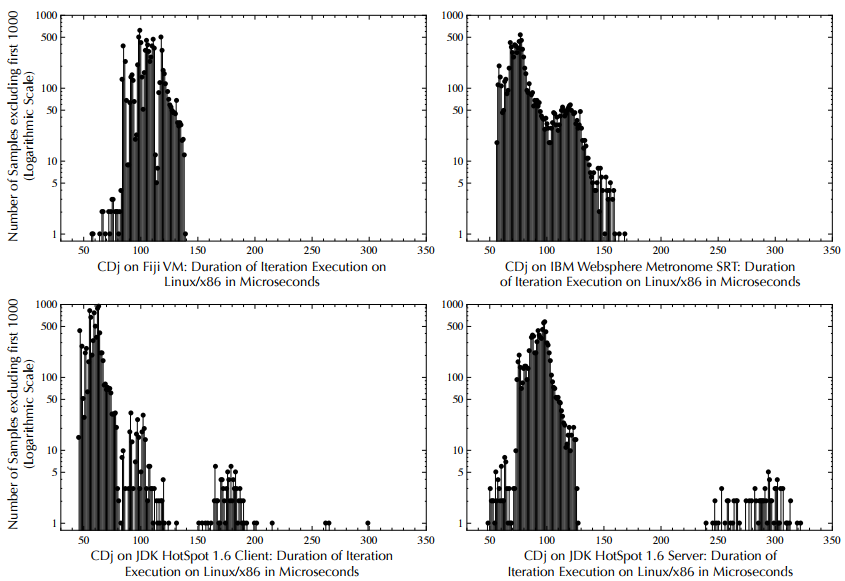
\includegraphics[width=0.8\linewidth]{images/fijicomp}
	\caption[Valutazione rispetto ad altre VM]{Valutazione di FijiVM rispetto ad altre VM}
	\label{fig:fijicomp}
\end{figure}

Si nota che Hotspot è decisamente più veloce rispetto a Fiji (37\% Server e 4.7\% Client), ma nel caso peggiore (quello realmente importante per sistemi real-time), Hotspot si comporta molto male (circa 185/200\% peggio di Fiji). Queste differenze sono causate dalle pause introdotte dalla GC, che non tiene conto della prevedibilità, ma cerca solo di ottimizzare il caso migliore. Rispetto a WebSphere, invece, Fiji si comporta meglio (nel caso peggiore) del 4\%, anche se in generale WebSphere è più veloce del 15\%. Tuttavia Fiji ha una distribuzione più stretta (calcolata rispetto alla differenza picchi/valli). Questo è un grande pregio, perché significa che la differenza tra il caso migliore e quello peggiore è più bassa.

Figura\ref{fig:fijistartup} mostra l'evoluzione del caso peggiore per diverse VM. Il grafico è in qualche modo simile a quello mostrato in Figura\ref{fig:performanceaotvsjit}. Hotspot e WebSphere utilizzano un compilatore JIT. Di conseguenza i tempo necessario al raggiungimento delle migliori prestazioni è variabile e più alto di quello di Fiji, che usa un compilatore AOT. Come detto precedentemente, le performance in generale saranno migliori per le altre VM (confermato da Figura\ref{fig:fijicomp}), ma il tempo necessario per raggiungere quei livelli è alto e riduce il determinismo.
\begin{figure}[h]
	\centering
	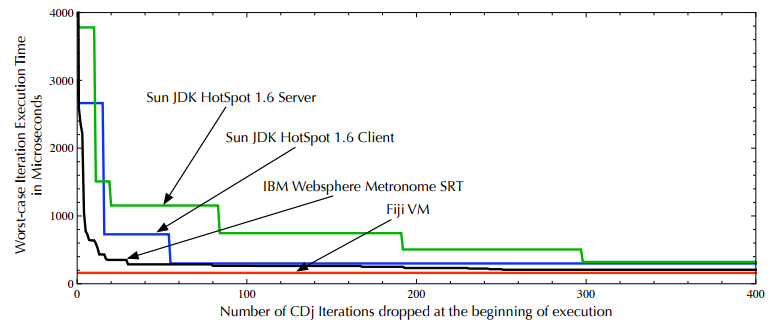
\includegraphics[width=0.8\linewidth]{images/fijistartup}
	\caption[Evoluzione del caso peggiore]{Evoluzione del caso peggiore per diverse VM}
	\label{fig:fijistartup}
\end{figure}
